\chapter{Schroedinger equation in 1d}
%
In this chapter we will be concentrating on the problem of
finding bound states solution to time-independent
Schroedinger equation in one dimension:
\begin{equation}
\left[ -\frac{1}{2}\frac{\mathrm{d}^2}{\mathrm{d}x^2} + V(x) \right] \psi(x) = E\, \psi(x)
\label{eq:Sch_1d_eq}
\end{equation}
%
with the boundary conditions:
%
\begin{equation}
\lim_{x \rightarrow \pm \infty} \psi(x) = 0
\label{eq:BC_isolated}
\end{equation}
%
This boundary condition is relevant for non-periodic systems such as
isolated or free atoms and molecules.

\section{Grid points}

We need to define a spatial domain $\left[x_{\mathrm{min}}, x_{\mathrm{max}}\right]$
where $x_{\mathrm{min}}, x_{\mathrm{max}}$ chosen
such that the boundary condition \ref{eq:BC_isolated} is approximately satisfied.
The next step is to divide the spatial domain $x$ using equally-spaced grid points
which we will denote as $\{x_{1},x_{2},\ldots,x_{N}\}$ where $N$ is total number
of grid points. Various spatial quantities such as wave function $\psi(x)$
and potential $\psi(x)$ will be discretized on these grid points.

The grid points $x_{i}$, $i = 1, 2, \ldots$ are chosen to be:
%
\begin{equation}
x_{i} = x_{\mathrm{min}} + (i-1)h
\end{equation}
%
where $h$ is the spacing between the grid points:
%
\begin{equation}
h = \frac{ x_{\mathrm{max}} - x_{\mathrm{min}} }{N-1}
\end{equation}

The following Julia function can be used to initialize the grid points.
\begin{juliacode}
function init_FD1d_grid( x_min::Float64, x_max::Float64, N::Int64 )
  L = x_max - x_min
  h = L/(N-1) # spacing
  x = zeros(Float64,N) # the grid points
  for i = 1:N
    x[i] = x_min + (i-1)*h
  end
  return x, h
end
\end{juliacode}
The function \jlinline{init_FD1d_grid} takes three arguments:
\begin{itemize}
\item \jlinline{x_min::Int64}: the left boundary point
\item \jlinline{x_max::Int64}: the right boundary point
\item \jlinline{N::Float64}: number of grid points
\end{itemize}
The function will return $x$ which is an array of grid points and $h$ which
is the uniform spacing between grid points. The boundary points \jlinline{x_min}
and \jlinline{x_max} will be included in the grid points.

As an example of the usage of the function \jlinline{init_FD1d_grid}, let's
sample and plot a Gaussian function
%
\begin{equation}
\psi(x) = \mathrm{e}^{-\alpha x^2}
\label{eq:gauss_func1}
\end{equation}
%
where $\alpha$ is a positive number. We will sample the function
within the domain $[x_{\text{min}},x_{\text{max}}]$ where
$x_{\text{min}}=-5$ and $x_{\text{max}}=5$.
The Gaussian function defined in \eqref{eq:gauss_func1} can be implemented
as the following function.
\begin{juliacode}
function my_gaussian(x::Float64; α=1.0)
  return exp( -α*x^2 )
end
\end{juliacode}
Note that we have set the default value of parameter $\alpha$ to 1.

The full Julia program is as follows.
%
\begin{juliacode}
using Printf
using LaTeXStrings

import PyPlot
const plt = PyPlot
plt.rc("text", usetex=true)

include("init_FD1d_grid.jl")

function my_gaussian(x::Float64; α=1.0)
  return exp( -α*x^2 )
end

function main()
  A = -5.0
  B =  5.0
  Npoints = 8
  x, h = init_FD1d_grid( A, B, Npoints )
  @printf("Grid spacing = %f\n", h)
  @printf("\nGrid points:\n")
  for i in 1:Npoints
    @printf("%3d %18.10f\n", i, x[i])
  end
  NptsPlot = 200
  x_dense = range(A, stop=5, length=NptsPlot)
  plt.clf()
  plt.plot(x_dense, my_gaussian.(x_dense), label=L"f(x)")
  plt.plot(x, my_gaussian.(x), label=L"Sampled $f(x)$", marker="o")
  plt.legend()
  plt.tight_layout()
  plt.savefig("IMG_gaussian_1d_8pt.pdf")
end
main()
\end{juliacode}

After execution, the program will print grid spacing and grid points to the standard
output and also plot the function to a file named \jlinline{IMG_gaussian_1d_8pt.pdf}
You may try to experiment by changing the value of \jlinline{N} and compare the result.
The resulting plots for \jlinline{N=8} and \jlinline{N=21} are shown in Figure XXX.
\begin{figure}[H]
{\center
\includegraphics[width=0.65\textwidth]{../codes/FD1d/IMG_gaussian_1d_8pt.pdf}
\includegraphics[width=0.65\textwidth]{../codes/FD1d/IMG_gaussian_1d_21pt.pdf}
\par}
\caption{Sampling a Gaussian function defined in \eqref{eq:gauss_func1}, $\alpha=1$,
two different number of grid points: $N=8$ (upper) and $N=21$ (lower). The sampled
coordinates are marked by dots. The true or "continuous" function is emulated by using
a dense sampling points of 200.}
\end{figure}

Note that we have used a densely-sampled points of \jlinline{NptsPlot=200} in the
program to emulate the true or "continuous" function. The plot of densely-sampled
array is not done by not showing the point marker, as opposed to the array with
lower sampling points.

\textbf{Exercise} Try to vary the value of $\alpha$ and \jlinline{N}.
Make the program more sophisticated
by using loop over for various values of \jlinline{N} instead of manually changing its value
in the program. You also may want to make set the saved filename of the resulting
plot programmatically.



\section{Approximating second derivative operator}

Our next task is to find an approximation to the second derivative operator
present in the Equation \eqref{eq:Sch_1d_eq}. Suppose that we have a function
sampled at appropriate positions $x_i$ as $\psi(x_{i})$. How can we approximate
$\psi''(x_{i})$ ?
One simple approximation that we can use is the 3-point (central) finite difference:
\begin{equation}
\frac{\mathrm{d}^2}{\mathrm{d}x^2} \psi_{i} =
\frac{\psi_{i+1} - 2\psi_{i} + \psi_{i-1}}{h^2}
\label{eq:fd_2nd_deriv_3pt}
\end{equation}
where we have the following notation have been used: $\psi_{i} = \psi(x_{i})$.
Let's see we can apply this by writing out the Equation \eqref{eq:fd_2nd_deriv_3pt}.
\begin{align*}
\psi''_{1} & \approx \left( \psi_{2} - 2\psi_{1} + \psi_{0} \right)/h^2 \\
\psi''_{2} & \approx \left( \psi_{3} - 2\psi_{2} + \psi_{1} \right)/h^2 \\
\psi''_{3} & \approx \left( \psi_{4} - 2\psi_{3} + \psi_{2} \right)/h^2 \\
& \vdots \\
\psi''_{N} & \approx \left( \psi_{N+1} - 2\psi_{N} + \psi_{N-1} \right)/h^2 \\
\end{align*}
In the first and the last equations, there are terms involving $\psi_{0}$ and
$\psi_{N+1}$ which are not known. Recall that we have numbered
our grid from 1 to $N$, so $\psi_{0}$ and $\psi_{N+1}$ are outside of our
grid. However, by using the boundary equation \eqref{eq:BC_isolated}, these
quantities can be taken as zeros. So we have:
\begin{align*}
\psi''_{1} & \approx \left( \psi_{2} - 2\psi_{1} \right)/h^2 \\
\psi''_{2} & \approx \left( \psi_{3} - 2\psi_{2} + \psi_{1} \right)/h^2 \\
\psi''_{3} & \approx \left( \psi_{4} - 2\psi_{3} + \psi_{2} \right)/h^2 \\
& \vdots \\
\psi''_{N} & \approx \left( - 2\psi_{N} + \psi_{N-1} \right)/h^2 \\
\end{align*}
This operation can be compactly expressed by using matrix-vector notation.
By taking $\{ \psi_{i} \}$ as a column vector, the second derivative operation
can be expressed as matrix multiplication:
\begin{equation}
\{ \psi'' \} \approx \mathbb{D}^{(2)} \{ \psi \}
\end{equation}
%%
where $\mathbb{D}^{(2)}$ is the second derivative matrix operator:
%
\begin{equation}
\mathbb{D}^{(2)} = \frac{1}{h^2}
\begin{bmatrix}
-2  &  1  &  0  &  0  & 0 & \cdots & 0 \\
 1  & -2  &  1  &  0  & 0 & \cdots & 0 \\
 0  &  1  & -2  &  1  & 0 & \cdots & 0 \\
 \vdots  &  \ddots  &  \ddots  & \ddots  & \ddots  & \ddots & \vdots \\
 0 & \cdots & 0 & 1 & -2 & 1 & 0 \\
 0  &  \cdots  & \cdots & 0  & 1  & -2  & 1 \\
 0  &  \cdots  & \cdots & \cdots & 0  &  1  & -2 \\
\end{bmatrix}
\label{eq:1d_D2_matmul}
\end{equation}

The following Julia function can be used to initialize the matrix $\mathbb{D}^{(2)}$.
\begin{juliacode}
function build_D2_matrix_3pt( N::Int64, h::Float64 )
  mat = zeros(Float64,N,N)1
  for i = 1:N-1
    mat[i,i] = -2.0
    mat[i,i+1] = 1.0
    mat[i+1,i] = mat[i,i+1]
  end
  mat[N,N] = -2.0
  return mat/h^2
end
\end{juliacode}
The function \jlinline{build_D2_matrix_3pt} takes two arguments:
\begin{itemize}
\item \jlinline{N::Int64}: number of grid points
\item \jlinline{h::Float64}: the uniform grid spacing
\end{itemize}
and returns the matrix $\mathbb{D}^{(2)}$ as two dimensional array.

Before use these functions to solve Schroedinger equation, we will test the operation
in Equation \eqref{eq:1d_D2_matmul} for a simple function for which the second derivative
can be calculated analytically. This function also should satisfy the boundary condition
\ref{eq:BC_isolated}. We will take the the Gaussian function
\eqref{eq:gauss_func1} that we have used before.
The second derivative of this Gaussian function can be calculated as
%
\begin{equation}
\psi''(x) = \left( -2 \alpha + 4\alpha^2 x^2 \right) \mathrm{e}^{-\alpha x^2}
\end{equation}

We also need to define the computational domain
$[x_{\text{min}},x_{\text{max}}]$ for our test.
Let's choose $x_{\text{min}} = -5$ and $x_{\text{max}} = 5$ again as in the previous example.
We can evaluate the value of function $\psi({x})$ at those points to be at the
order of $10^{-11}$, which is sufficiently small for our purpose.

The full Julia program that we will use is as follows.
\begin{juliacode}
using Printf
using LaTeXStrings

import PyPlot
const plt = PyPlot
plt.rc("text", usetex=true)

include("init_FD1d_grid.jl")
include("build_D2_matrix_3pt.jl")

function my_gaussian(x, α=1.0)
  return exp(-α*x^2)
end

function d2_my_gaussian(x, α=1.0)
  return (-2*α + 4*α^2 * x^2) * exp(-α*x^2)
end

function main(N::Int64)
  x_min = -5.0
  x_max =  5.0
  x, h = init_FD1d_grid( x_min, x_max, N )
  fx = my_gaussian.(x)

  Ndense = 200
  x_dense = range(A, stop=B, length=Ndense)
  fx_dense = my_gaussian.(x_dense)
  d2_fx_dense = d2_my_gaussian.(x_dense)

  D2 = build_D2_matrix_3pt(N, h)
  d2_fx_3pt = D2*fx

  plt.clf()
  plt.plot(x, fx, marker="o", label=L"Sampled $f(x)$")
  plt.plot(x_dense, fx_dense, label=L"f(x)")
  plt.plot(x, d2_fx_3pt, marker="o", label=L"Approx $f''(x)$")
  plt.plot(x_dense, d2_fx_dense, label=L"f''(x)")
  plt.legend()
  plt.grid()
  plt.savefig("IMG_gaussian_"*string(N)*".pdf")
end
main(15)
main(51)
\end{juliacode}

We have followed similar approach as we have done in the previous section for plotting.
The important parts of the program are the lines:
\begin{juliacode}
D2 = build_D2_matrix_3pt(N, h)
d2_fx_3pt = D2*fx
\end{juliacode}
where we build $\mathbb{D}^{(2)}$ matrix, represented by the variable
\jlinline{D2} in the program, and multiply it with the vector \jlinline{fx}
to obtain an approximation to $\psi''(x)$. The results are plotted with two
different values of number of grid points, $\jlinline{N=15}$ and $\jlinline{N=51}$,
which are shown in Figure XXX.

\begin{figure}[H]
{\center
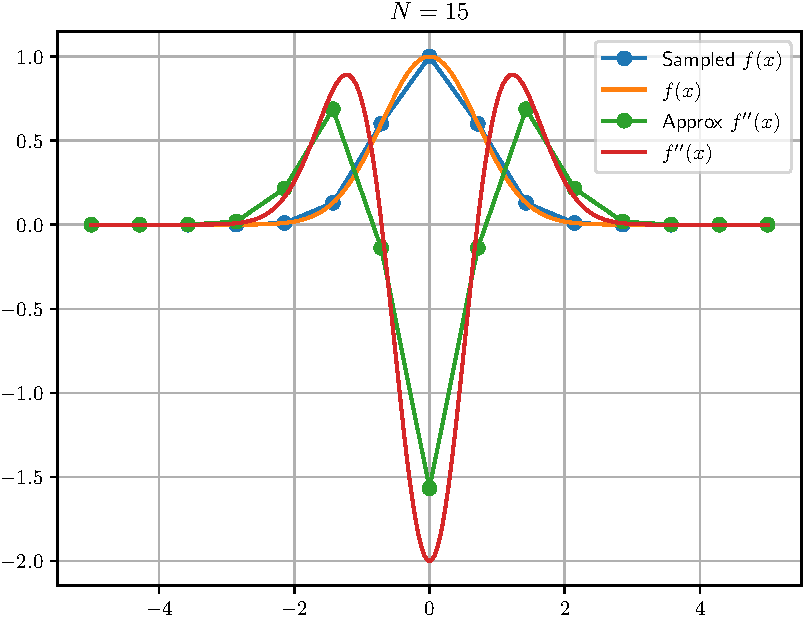
\includegraphics[width=0.65\textwidth]{../codes/FD1d/IMG_gaussian_15.pdf}
\par}
\caption{Finite difference approximation to a Gaussian function and its second derivative with
number of grid points $N=15$}
\end{figure}

\begin{figure}[H]
{\center
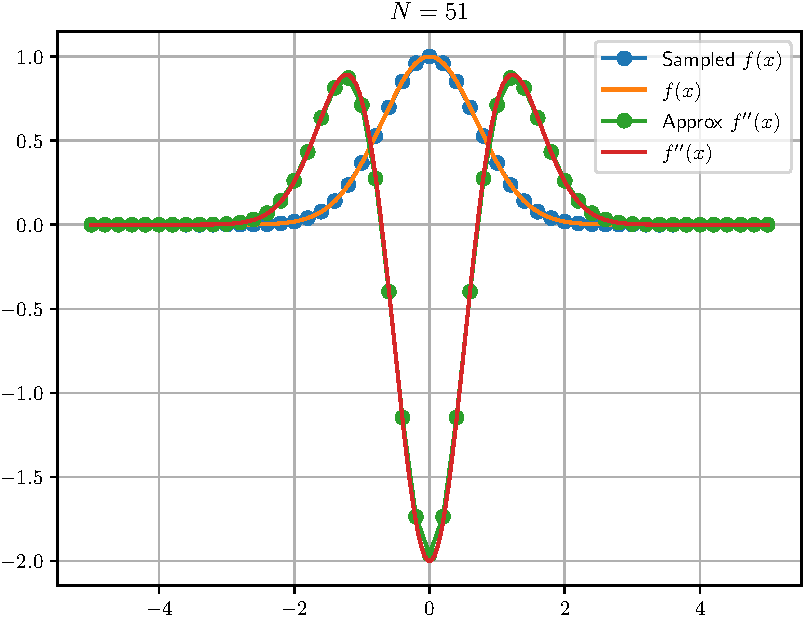
\includegraphics[width=0.65\textwidth]{../codes/FD1d/IMG_gaussian_51.pdf}
\par}
\caption{Finite difference approximation to a Gaussian function and its second derivative with
number of grid points $N=51$}
\end{figure}


\section{Harmonic potential}

The time-independent Schroedinger equation \eqref{eq:Sch_1d_eq} can be expressed into
the following eigenvalue problem in matrix form:
\begin{equation}
\mathbb{H}\{ \psi \} = E \{ \psi \}
\end{equation}
where $\mathbb{H}$ is the Hamiltonian matrix and $\{ \psi \}$ is a vector
column representation of wave function.
In finite difference representation, the Hamiltonian matrix is
\begin{equation}
\mathbb{H} = -\frac{1}{2}\mathbb{D}^{(2)} + \mathbb{V}
\end{equation}
where $\mathbb{V}$ is a diagonal matrix whose elements are:
\begin{equation}
\mathbb{V}_{ij} = V(x_{i})\delta_{ij}
\end{equation}

As an example, we will start with a simple potential with known exact solution,
namely the harmonic potential:
\begin{equation}
V(x) = \frac{1}{2}\omega^2 x^2
\end{equation}

In Julia, we can the process of building the Hamiltonian matrix is very simple
\begin{juliacode}
x, h = init_FD1d_grid(xmin, xmax, N) # grid points
D2 = build_D2_matrix_3pt(N, h)       # Build 2nd derivative matrix
Vpot = pot_harmonic.(x)              # Potential
Ham = -0.5*D2 + diagm( 0 => Vpot )   # Hamiltonian matrix
\end{juliacode}

The function \jlinline{pot_harmonic} is a function that calculate the harmonic potential
\begin{juliacode}
function pot_harmonic( x; ω=1.0 )
  return 0.5 * ω^2 * x^2
end
\end{juliacode}

Once the Hamiltonian matrix is built, we can solve for $E$ and $\{\psi\}$ by using standard
methods. In Julia this can be achieved by simply using the \jlinline{eigen} function
from \jlinline{LinearAlgebra} standard library as illustrated in the following code.
\begin{juliacode}
evals, evecs = eigen( Ham )
\end{juliacode}
The values of $E$ or eigenvalues are stored in one-dimensional array \jlinline{evals}
and the corresponding wave functions or eigenvectors are stored by column in two-dimensional
array or matrix \jlinline{evecs}.

The complete Julia program to solve the Schroedinger equation for harmonic potential
is as follows.

\begin{juliacode}
using Printf
using LinearAlgebra
using LaTeXStrings
  
import PyPlot
const plt = PyPlot
plt.rc("text", usetex=true)

include("init_FD1d_grid.jl")
include("build_D2_matrix_3pt.jl")
  
function pot_harmonic( x; ω=1.0 )
  return 0.5 * ω^2 * x^2
end
  
function main()
  xmin = -5.0
  xmax =  5.0
  N = 51
  x, h = init_FD1d_grid(xmin, xmax, N)
  D2 = build_D2_matrix_3pt(N, h)
  Vpot = pot_harmonic.(x)
  Ham = -0.5*D2 + diagm( 0 => Vpot )
  evals, evecs = eigen( Ham )
  # We will show the 5 lowest eigenvalues
  Nstates = 5
  @printf("Eigenvalues\n")
  ω = 1.0
  hbar = 1.0
  @printf(" State         Approx              Exact          Difference\n")
  for i in 1:Nstates
    E_ana = (2*i - 1)*ω*hbar/2
    @printf("%5d %18.10f %18.10f %18.10e\n", i, evals[i], E_ana, abs(evals[i]-E_ana))
  end
  
  # normalize the first three eigenstates
  for i in 1:3
    ss = dot(evecs[:,i], evecs[:,i])*h
    evecs[:,i] = evecs[:,i]/sqrt(ss)
  end
  
  # Plot up to 3rd eigenstate
  plot_title = "N="*string(N)
  plt.plot(x, evecs[:,1], label="1st eigenstate", marker="o")
  plt.plot(x, evecs[:,2], label="2nd eigenstate", marker="o")
  plt.plot(x, evecs[:,3], label="3rd eigenstate", marker="o")
  plt.legend()
  plt.grid()
  plt.tight_layout()
  plt.savefig("IMG_main_harmonic_01_"*string(N)*".pdf")
end

main()
\end{juliacode}

The program shows five lowest approximate eigenvalues and their comparison with analytical or
exact eigenvalues. A sample output from running the program is as follows.
\begin{textcode}
Eigenvalues
State         Approx              Exact          Difference
   1       0.4987468513       0.5000000000   1.2531486828e-03
   2       1.4937215179       1.5000000000   6.2784821079e-03
   3       2.4836386480       2.5000000000   1.6361352013e-02
   4       3.4684589732       3.5000000000   3.1541026791e-02
   5       4.4481438504       4.5000000000   5.1856149551e-02 
\end{textcode}

The program will also plot three lowest resulting eigenvectors (wave functions) to a file.
An example plot is show in Figure \ref{fig:wfn_harm_01_51}.

\begin{figure}[H]
{\center
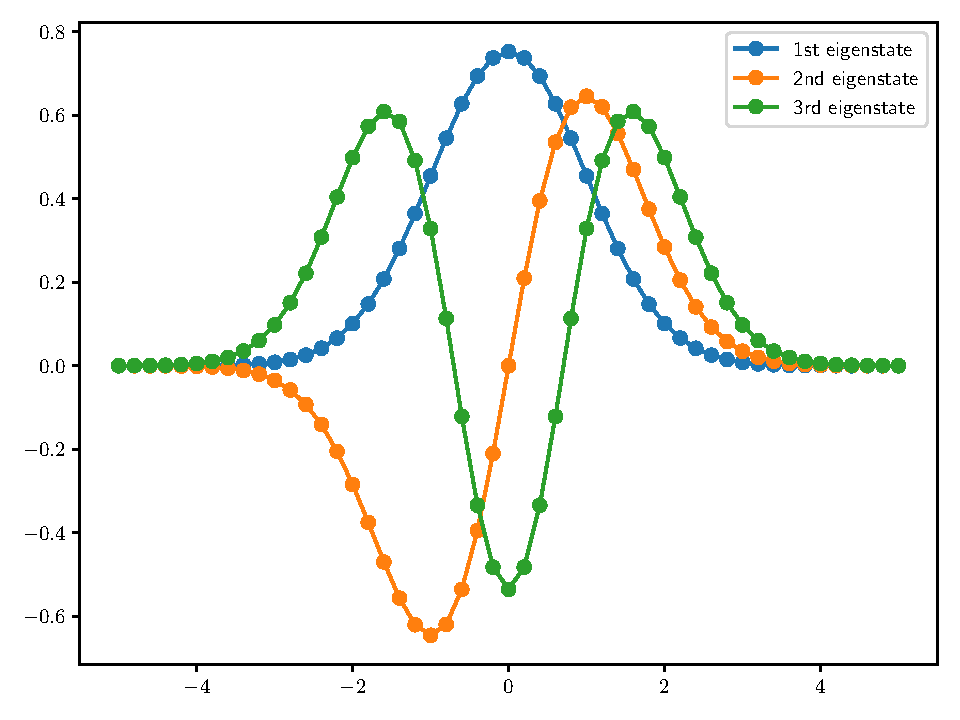
\includegraphics[scale=0.65]{../codes/sch_1d/IMG_main_harmonic_01_51.pdf}
\par}
\caption{Eigenstates of harmonic oscillator}
\label{fig:wfn_harm_01_51}
\end{figure}

You can get more accurate values of eigenvalues by using higher value for grid points.
This is the result if we use $N=81$.
\begin{textcode}
Eigenvalues
State         Approx              Exact          Difference
   1       0.4995112405       0.5000000000   4.8875946328e-04
   2       1.4975542824       1.5000000000   2.4457175928e-03
   3       2.4936355672       2.5000000000   6.3644328157e-03
   4       3.4877496130       3.5000000000   1.2250387024e-02
   5       4.4798939398       4.5000000000   2.0106060206e-02 
\end{textcode}


\section{Higher order finite difference}

To obtain higher accuracy, we can include more points in our approximation to second
derivative operator. An example is by using 5-point finite-difference formula:
\begin{equation}
\frac{\mathrm{d}^2}{\mathrm{d}x^2} \psi_{i} =
\frac{-\psi_{i+2} + 16\psi_{i+1} - 30\psi_{i} + 16\psi_{i-1} - \psi_{i-2}}{12h^2}
\label{eq:fd_2nd_deriv_5pt}
\end{equation}

The corresponding second derivative matrix can be built using the following
function.
\begin{juliacode}
function build_D2_matrix_5pt( N::Int64, h::Float64 )
  mat = zeros(Float64,N,N)
  for i = 1:N-2
    mat[i,i] = -30.0
    mat[i,i+1] = 16.0
    mat[i,i+2] = -1.0
    mat[i+1,i] = mat[i,i+1]
    mat[i+2,i] = mat[i,i+2]
  end
  #
  mat[N-1,N-1] = -30.0
  mat[N-1,N] = 16.0
  mat[N,N-1] = mat[N-2,N-1]
  mat[N,N] = -30.0
  #
  return mat/(12*h^2)
end
\end{juliacode}

We will refer to the number of points used to approximate the derivative operator as
stencil order, thus the Equation \eqref{eq:fd_2nd_deriv_5pt} has stencil order of 5
and Equation \eqref{eq:fd_2nd_deriv_3pt} has stencil order of 3.
Other approximation formulas for second derivative also can be used.
In the source code reposityory, we have implemented 3-,
5-, 7-, 9-, and 11-points formulas. The web page
{\footnotesize\url{http://web.media.mit.edu/~crtaylor/calculator.html}}
can be consulted to obtain the
coefficients of finite-difference approximation.

In Figure \ref{fig:fd_2nd_compare_N15} we plot the difference (approximation - exact)
of second derivative of
the Gaussian function for several approximation formulas using $N=15$ grid points.
The errors have have different magnitude for each points with the maximum error
occurs at the center of the Gaussian.
We can readily see that the errors for each point are decreasing with increasing stencil
order.
\begin{figure}[h]
{\center
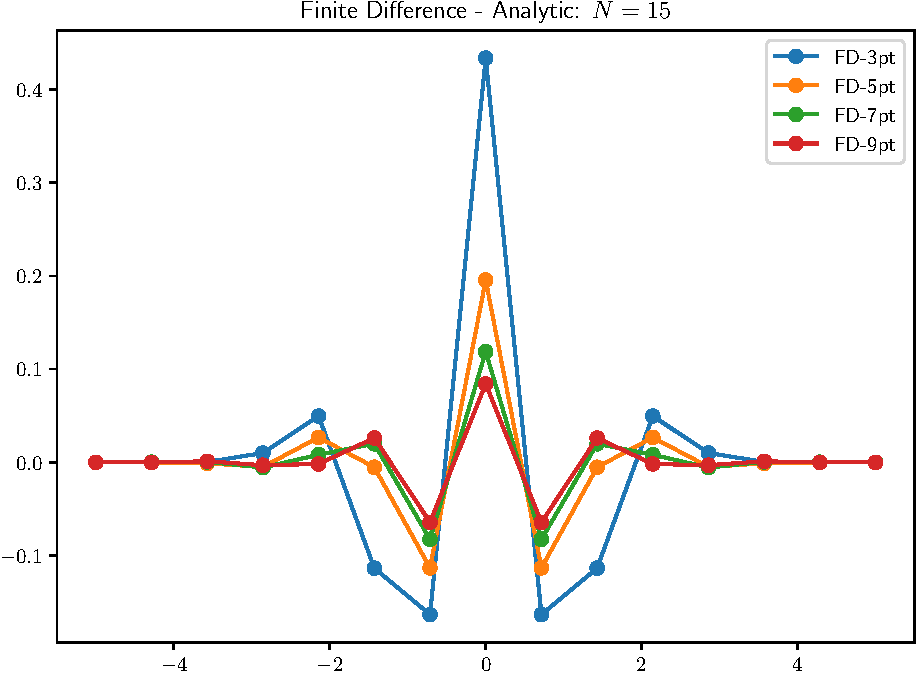
\includegraphics[width=0.65\textwidth]{../codes/FD1d/IMG_compare_d2_gaussian_error_15.pdf}
\par}
\caption{Error of 2nd derivative approx}
\label{fig:fd_2nd_compare_N15}
\end{figure}


\section{Harmonic potential with higher order finite-difference formulas}

We can compare the effect of different stencil order to the accuracy of numerical approximation
to the Schroedinger equation. In the following program, we try to compare the accuracy of
first eigenvalue of Schroedinger equation with harmonic potential.

\begin{juliacode}
function solve_eigvals(N::Int64, D2_func)
  # Initialize the grid points
  x_min = -5.0
  x_max =  5.0
  x, h = init_FD1d_grid(x_min, x_max, N)
  # Build 2nd derivative matrix
  D2 = D2_func(N, h)
  # Potential
  Vpot = pot_harmonic.(x)
  # Hamiltonian
  Ham = -0.5*D2 + diagm( 0 => Vpot )
  # Solve for the eigenvalues only
  evals = eigvals( Ham )
  #
  return evals
end

function main()
  Npoints = 20
  funcs = [build_D2_matrix_3pt, build_D2_matrix_5pt, build_D2_matrix_7pt,
           build_D2_matrix_9pt, build_D2_matrix_11pt]

  ω = 1.0
  hbar = 1.0
  ist = 1
  E_ana = (2*ist - 1)*ω*hbar/2

  for f in funcs
      evals = solve_eigvals(Npoints, f)
      dE = abs(evals[ist]-E_ana) # absolute error
      @printf("%20s: %18.10f %18.10e\n", string(f), evals[ist], dE)
  end
end

main()
\end{juliacode}

The results for fixed point ($N=20$) and different stencil order are given below.
The second colum is the first eigenvalue and the third colum in the difference with
exact value (0.5 Hartree). The results clearly shows that the error decreases with
with increasing stencil order.

\begin{textcode}
  build_D2_matrix_3pt:       0.4911851752   8.8148248058e-03
  build_D2_matrix_5pt:       0.4992583463   7.4165366457e-04
  build_D2_matrix_7pt:       0.4998965249   1.0347512122e-04
  build_D2_matrix_9pt:       0.4999802170   1.9782954165e-05
 build_D2_matrix_11pt:       0.4999952673   4.7326636594e-06
\end{textcode}

\section{Exercises}

Potential well

Gaussian potential


\textbf{Periodic boundary condition}

Let the potential $V(x)$ be a periodic function:
\begin{equation}
V(x) = V(x + jL)
\end{equation}
where $j = 0, 1, 2, \ldots$ and $L$ is the periodicity of the potential.
Using Bloch theorem, the solution $\psi_{k}(x)$ of the Schroedinger equation
can be written as
\begin{equation}
\psi_{k}(x) = e^{\imath k x} \phi_{k}(x)
\end{equation}
where $\phi_{k}$ dan its first derivative have the same periodicity as $V(x)$.
Show that in terms of $\phi_{k}$ the Schroedinger equation can be written as:
\begin{equation}
\left[
-\frac{\hbar^2}{2m}\left( \frac{\mathrm{d}^2}{\mathrm{d}x^2} +
2\imath k \frac{\mathrm{d}}{\mathrm{d}x} - k^2
\right) + V(x) \right] \phi_{k}(x) = E \phi_{k}(x)
\end{equation}
Solve for and plot the solution $E(k)$ (dispersion relation) for the following
periodic potentials:
\begin{itemize}
\item Kronig-Penney potential:
\begin{equation}
V(x) = \begin{cases}
V_{0} & x \geq L/4 \, \text{and} \, x \leq 3L/4 \\
0 \, \text{otherwise} \\
\end{cases}
\end{equation}
%
\item Mathieu potential
\begin{equation}
V(x) = V_{0} \left( 1 + \cos\left(\frac{2\pi x}{L}\right) \right)
\end{equation}
\end{itemize}
